\section{Методика коррекции динамических свойств КЭ-модели}

\begin{frame}{Методика коррекции конечно-элементной модели}
	\begin{block}{Обобщенная проблема собственных значений}
		\begin{equation}
			(\mat{K} - \lambda \mat{M}) \mat{Y} = 0,
		\end{equation}
		где $ \mat{K} $, $ \mat{M} \in \set{R} ^ {n \times n}$~---~матрицы жесткости и масс; $ \mat{Y} $~---~формы собственных колебаний; $ \lambda $~---~собственные числа; $ N $~---~число степеней свободы.
	\end{block}
	\begin{block}{Корректирующая матрица жесткости в общем виде}
 		\begin{equation}
 			\begin{gathered}
 				\Delta \mat{K} = \Delta \internal{\mat{K}} + \Delta \external{\mat{K}}, \\
				\Delta \internal{\mat{K}}_j = \sum\limits_{p\,=\,1}^{q} \internal{c}_{j+p-1} \mat{G}_j^{(p)}, \ j = 1 \hdots e, \\
				\Delta \external{\mat{K}} = \operatorname{diag} \cbrackets{\external{c}_1, \external{c}_2, \hdots, \external{c}_N}.
			\end{gathered}
		\end{equation}
		где $ \internal{\mat{c}} $ и $ \external{\mat{c}} $~---~внутренние и внешние корректирующие жесткости; $ q $~---~число внутренних парциальных корректирующих жесткостей, описывающих элемент; $ \mat{G}_j^{(p)} $~---~парциальная матрица жесткости внутреннего коррректирующего элемента; $ e $~---~число внутренних корректирующих элементов.
	\end{block}
\end{frame}

\begin{frame}{Внутренний корректирующий элемент в виде балки}
	\begin{block}{Парциальные корректирующие матрицы жесткости}
		\begin{equation*}
		\begingroup
		\setlength\arraycolsep{2pt}
		\begin{gathered}
			\mat{G}_j^{(1)} =
			\begin{pmatrix}
				\mat{D}_1 & \mat{0} & -\mat{D}_1 & \mat{0} \\
				\mat{0} & \mat{0} & \mat{0} & \mat{0} \\
				-\mat{D}_1 & \mat{0} & \mat{D}_1 & \mat{0} \\
				\mat{0} & \mat{0} & \mat{0} & \mat{0} \\
			\end{pmatrix},
			\mat{G}_j^{(2)} =
			\begin{pmatrix}
				6 \mat{D}_2 & 3 \ell \mat{D}_4 & -6 \mat{D}_2 & 3 \ell \mat{D}_4 \\
				3 \ell \trans{\mat{D}}_4 & 2 \ell ^ 2 \mat{D}_3 & -3 \ell \trans{\mat{D}}_4 & \ell ^ 2 \mat{D}_3 \\
				-6 \trans{\mat{D}}_2 & -3 \ell \mat{D}_4 & 6 \mat{D}_2 & -3 \ell \mat{D}_4 \\
				3 \ell \trans{\mat{D}}_4 & \ell ^ 2 \trans{\mat{D}}_3 & -3 \ell \trans{\mat{D}}_4 & 2 \ell ^ 2 	\mat{D}_3
			\end{pmatrix}, \\
			\mat{G}_j^{(3)} =
			\begin{pmatrix}
				6 \mat{D}_3 & -3 \ell \trans{\mat{D}}_4 & -6 \mat{D}_3 & -3 \ell \trans{\mat{D}}_4 \\
				-3 \ell \mat{D}_4 & 2 \ell ^ 2 \mat{D}_2 & 3 \ell \mat{D}_4 & \ell ^ 2 \mat{D}_2 \\
				-6 \trans{\mat{D}}_3 & 3 \ell \trans{\mat{D}}_4 & 6 \mat{D}_3 & 3 \ell \trans{\mat{D}}_4 \\
				-3 \ell \mat{D}_4 & \ell ^ 2 \trans{\mat{D}}_2 & 3 \ell \mat{D}_4 & 2 \ell ^ 2 \mat{D}_2
			\end{pmatrix},
			\mat{G}_j^{(4)} =
			\begin{pmatrix}
				\mat{0} & \mat{0} & \mat{0} & \mat{0} \\
				\mat{0} & \mat{D}_1 & 0 & -\mat{D}_1 \\
				\mat{0} & \mat{0} & \mat{0} & \mat{0} \\
				\mat{0} & -\mat{D}_1 & 0 & \mat{D}_1 \\
			\end{pmatrix},
		\end{gathered}
		\endgroup
		\end{equation*}
	\end{block}
	\begin{block}{Матрицы из направляющих косинусов}
		\begin{equation*}
			\mat{D}_k = 
			\begin{pmatrix}
				d_{k, 1}^2 & d_{k, 1} d_{k, 2} & d_{k, 1} d_{k, 3} \\
				d_{k, 2} d_{k, 1} & d_{k, 2} ^ 2 & d_{k, 2} d_{k, 3} \\
				d_{k, 3} d_{k, 1} & d_{k, 3} d_{k, 2} & d_{k, 3} ^ 2
				\end{pmatrix},
			\mat{D}_4 = 
			\begin{pmatrix}
				d_{2, 1} d_{3, 1} & d_{2, 1} d_{3, 2} & d_{2, 1} d_{3, 3} \\
				d_{2, 2} d_{3, 1} & d_{2, 2} d_{3, 2} & d_{2, 2} d_{3, 3} \\
				d_{2, 3} d_{3, 1} & d_{2, 3} d_{3, 2} & d_{2, 3} d_{3, 3}
			\end{pmatrix},
		\end{equation*}
	\end{block}
	где $ \ell $~---~длина корректирующего балочного элемента, $ k = 1 \hdots 3 $.
\end{frame}

\begin{frame}{Принципиальная схема коррекции}
	\centering
	\begin{tikzpicture}[scale = 1]
		\pgfmathsetmacro{\nodeDist}{0.1}
		\pgfmathsetmacro{\shiftText}{0.0}
		% Исходная модель
		\node[inner sep = 0pt] (initial) at (0, 0) {\includegraphics[width = 0.4\textwidth]{simple-model-initial}};
		\node[inner sep = 0pt, below = \shiftText of initial.south] (textInitial) {Исходная модель};
		% Знак
		\node [below = \nodeDist of textInitial.south, color = blue] (sumSign) {\huge \bfseries +};
		% Коррректирующие элементы
		\node[inner sep = 0pt, below = -\nodeDist of sumSign.south] (elements) {\includegraphics[width = 0.4\textwidth]{simple-model-elements}};
		\node[inner sep = 0pt, below = \shiftText of elements.south] (textElements) {Корректирующие элементы};
		% Скорректированная модель
		\draw [-{Latex[length = 4mm]}, color = red, very thick](sumSign.east) ++ (2, 0) --++ (1, 0) node [right] (updated) {\includegraphics[width = 0.5\textwidth]{simple-model-updated}};
		\node[inner sep = 0pt, below = \shiftText of updated.south] (textUpdated) {Скорректированная модель};
	\end{tikzpicture}
\end{frame}

\begin{frame}{Расчет корректирующих жесткостей}
	\begin{block}{Задача безусловной минимизации}
		\vspace{-1em}
		\begin{gather}
			f_j(c) = \mat{Y}_j^{(0)\mathsf{T}} \Delta \mat{K}^{(i+1)} \mat{Y}_j^{(i)} + \mat{Y}_j^{(0)\mathsf{T}} \mat{K} \Delta \mat{Y}_j^{(i)} - \Delta \lambda^*_j, \\
			F(c) = \sum \limits_{j\,=\,1}^s w_j f_j^2(c) + w_c \sum \limits_{k\,=\,1}^m c_k^2 \rightarrow \min_{c},
		\end{gather}
		где $ i $~---~номер текущей итерации, $ \Delta \lambda^*_j = \lambda_j^* - \lambda_{j0} $ ($\lambda_j^*$~---~целевые собственные значения), $ w_j $~---~весовые коэффициенты, $ s $~---~число целевых частот, $ w_c $~---~параметр регуляризации.
	\end{block}	
	\begin{block}{Нормировка собственных векторов}
		\vspace{-1em}
		\begin{gather}
			\mat{Y}^{(0)\mathsf{T}} \mat{M} \mat{Y}^{(0)} = 1, \\
			\mat{Y}^{(0)\mathsf{T}} \mat{M} \mat{Y}^{(i)} = 1 \Longrightarrow \mat{Y}^{(0)T} \mat{M} \Delta \mat{Y}^{(i)} = 0,
		\end{gather}
		где $ \mat{Y}^{(0)} $, $ \mat{Y}^{(i)} $~---~исходные и текущие собственные вектора.
	\end{block}	
\end{frame}

\begin{frame}{Формирование матрицы демпфирования в физической системе координат}
	\begin{block}{Нулевое приближение (гипотеза Е.\,C.~Сорокина)}
		\begin{gather}
			\mat{H} = \alpha \tilde{\mat{K}} + \beta \mat{M}, \\
			G(\alpha, \beta) = \sum\limits_{i\,=\,1}^p w_i \left( 1 - \frac{\alpha \tilde{\kappa}_i + \beta \mu_i}{h_i} \right)^2 \rightarrow \min_{\alpha, \beta},
		\end{gather}
		где $ \alpha $ и $ \beta $~---~коэффициенты конструкционного и инерционного демпфирования, $ h $~---~целевые обобщенные коэффициенты демпфирования, $ p $~---~число целевых коэффициентов.
	\end{block}
	\begin{block}{Преобразование матрицы демпфирования} 
 		\begin{equation} 
			\tilde{\mat{H}} = \mat{H} + \Delta \internal{\mat{H}} + \Delta \external{\mat{H}},
		\end{equation}
		где $ \Delta \internal{\mat{H}} $ и $ \Delta \external{\mat{H}} $~---~матрицы демпфирования внутренних и внешних корректирующих элементов. 
	\end{block}
\end{frame}

\begin{frame}{Методика освобождения КЭ-модели от закреплений}
	\begin{equation} 
		\begin{pmatrix}
			\mat{K} & -(\sum k)^\intercal \\
			 -\sum k & \mat{0} 
		\end{pmatrix} 
		\begin{Bmatrix}
			\tilde{X} \\ 
			\xi
		\end{Bmatrix}			
		+ 
		\begin{pmatrix}
			\mat{M} & \mat{0} \\
			\mat{0} & \mu - \sum \sum m
		\end{pmatrix}
			\begin{Bmatrix}
			\ddot{\tilde{\mat{X}}} \\ 
			\ddot{\mat{\xi}}
		\end{Bmatrix}	
		= 0,
	\end{equation}
	\begin{itemize}
		\item $ \mat{K}, \mat{M} \in R ^ {n \times n} $~---~матрицы жесткости и масс закрепленной модели,
		\item $ \mu \in R^{6 \times 6} $~---~матрица инерции,
		\item $ \xi $~---~вектор перемещений как жесткого целого,
		\item $ \tilde{\mat{X}} $~---~вектор перемещений свободной модели,
		\item $ \sum k = F_s(\mat{K}) \in R ^ {6 \times n}$, $ \sum \sum m = F_m(F_s(\mat{M})) \in R ^ {6 \times 6} $~{\footnotemark}.
	\end{itemize}
	\vfill
	\footnotetext[1]{Матричные функции $ F_s,\ F_m $ представлены на следующем слайде.}
\end{frame}

\begin{frame}{Матричные функции $ F_m $ и $ F_s $}
	\begingroup
	\setlength\arraycolsep{2pt}
	\begin{gather*}
		\small
		F_m(\mat{A})
		= \left(
		\begin{matrix}
			\sum \limits_{i=1}^N a_{1,G_{i,1}} 
			& \hdots
			& \sum \limits_{i=1}^N a_{1,G_{i,3}} 
			&
			\sum\limits_{i=1}^N
			\left(
			\begin{matrix}
				a_{1,G_{i,4}} + \\
				+ \Delta y_i^0 a_{1, G_{i,3}} - \\
				- \Delta z_i^0 a_{1, G_{i,2}} \\
			\end{matrix} \right)
			& 
			\hdots
			&
			\sum\limits_{i=1}^N
			\left(
			\begin{matrix}
				a_{1,G_{i,6}} + \\
				+ \Delta x_i^0 a_{1, G_{i,2}} - \\
				- \Delta y_i^0 a_{1, G_{i,1}} \\
			\end{matrix} \right) \\ 
			\hdots & \hdots & \hdots & \hdots & \hdots & \hdots \\
			\sum \limits_{i=1}^N a_{6,G_{i,1}} 
			& \hdots 
			& \sum \limits_{i=1}^N a_{6,G_{i,3}} 
			&
			\sum\limits_{i=1}^N
			\left(
			\begin{matrix}
				a_{6,G_{i,4}} + \\
				+ \Delta y_i^0 a_{6, G_{i,3}} - \\
				- \Delta z_i^0 a_{6, G_{i,2}} \\
			\end{matrix} \right)
			& 
			\hdots
			&
			\sum\limits_{i=1}^N
			\left(
			\begin{matrix}
				a_{6,G_{i,6}} + \\
				+ \Delta x_i^0 a_{6, G_{i,2}} - \\
				- \Delta y_i^0 a_{6, G_{i,1}} \\
			\end{matrix} \right) \\ 
		\end{matrix}
		\right), \\ 
		\small
		F_s(\mat{A}) ^ \intercal
		= \left(
		\begin{matrix}	
			\sum \limits_{i=1}^N a_{G_{i,1}, 1} 
			& \hdots 
			& \sum \limits_{i=1}^N a_{G_{i,3}, 1} 
			&
			\sum\limits_{i=1}^N
			\left(
			\begin{matrix}
				a_{G_{i,4}, 1} + \\
				+ \Delta y_i^0 a_{G_{i,3}, 1} - \\
				- \Delta z_i^0 a_{G_{i,2}, 1} \\
			\end{matrix} \right)
			& 
			\hdots
			&
			\sum\limits_{i=1}^N
			\left(
			\begin{matrix}
				a_{G_{i,6}, 1} + \\
				+ \Delta x_i^0 a_{G_{i,2}, 1} - \\
				- \Delta y_i^0 a_{G_{i,1}, 1} \\
			\end{matrix} \right) \\ 
			\hdots & \hdots & \hdots & \hdots & \hdots & \hdots \\
			\sum \limits_{i=1}^N a_{G_{i,1},n} 
			& \hdots
			& \sum \limits_{i=1}^N a_{G_{i,3},n} 
			&
			\sum\limits_{i=1}^N
			\left(
			\begin{matrix}
				a_{G_{i,4},n} + \\
				+ \Delta y_i^0 a_{G_{i,3}, n} - \\
				- \Delta z_i^0 a_{G_{i,2}, n} \\
			\end{matrix} \right)	
			& 
			\hdots
			&
			\sum\limits_{i=1}^N
			\left(
			\begin{matrix}
				a_{G_{i,6}, n} + \\
				+ \Delta x_i^0 a_{G_{i,2}, n} - \\
				- \Delta y_i^0 a_{G_{i,1}, n} \\
			\end{matrix} \right) \\ 
		\end{matrix}
		\right),
	\end{gather*}
	\endgroup
	где $ G_{i, j} $~---~номер уравнения $ i $-го узла $ j $-ой степени свободы; $ a_{i,j}$~---~элементы матрицы $ \mat{A} $; $ \Delta x^0_i, \Delta y^0_i, \Delta z^0_i $~---~компоненты радиус-вектора от центра тяжести до $ i $-го узла недеформированной конструкции.
\end{frame}

\section{Оценка чувствительности методики коррекции}

\begin{frame}{Оценка чувствительности методики коррекции}
	\textbf{\underline{Цель}}: оценка влияния погрешностей в экспериментальном определении частот на устойчивость результата коррекции. \\
	\textbf{\underline{Алгоритм}}
	\begin{enumerate}
		\item Вычисление частот и форм собственных колебаний исходной модели.
		\item Варьирование числа корректируемых тонов собственных колебаний и внесение случайных отклонений $ \Delta \mat{f} \sim \set{N} \rbrackets{\mu, \sigma ^ 2} $ в значения частот. 
		\item Решение задачи коррекции. Определение максимальной погрешности критерия модального соответствия $ \varepsilon_{\mathrm{MAC}} $ между исходными и полученными формами колебаний.
		\item Оценка первого центрального момента $ \mu_1\rbrackets{\varepsilon_{\mathrm{MAC}}} $ в зависимости от числа независимых испытаний с целью получения достоверных оценок математического ожидания и дисперсии. 
		\item Последовательность шагов 2~--~4 повторяется до тех пор, пока $ \mu_1\rbrackets{\varepsilon_{\mathrm{MAC}}} $, рассчитанный для выборки из последних наблюдений, не стабилизируется с заданной точностью.
	\end{enumerate}
\end{frame}

\begin{frame}{Оценка чувствительности на примере свободной прямоугольной пластины}
	\begin{center}	
		\begin{columns}
			\begin{column}{0.5\textwidth}
				\centering
				\begin{figure}
					\includegraphics[width = 1\textwidth]{perturbation-plate-convergence}
					\caption{Погрешность определения форм колебаний в зависимости от погрешности целевых частот}
				\end{figure}
			\end{column}
			\begin{column}{0.5\textwidth}
				\centering
				\vspace{-0.9em}
				\begin{figure}
					\includegraphics[width = 1\textwidth]{perturbation-plate-samplesize}
					\caption{Число независимых испытаний в зависимости от погрешности целевых частот}
				\end{figure}
			\end{column}
		\end{columns}
	\end{center}
\end{frame}

\section{Методика синтеза глобальных расчетных моделей конструкций}

\begin{frame}{Методика синтеза глобальных расчетных моделей конструкций}
	\begin{columns}
		\begin{column}{0.5\textwidth}
			\centering
			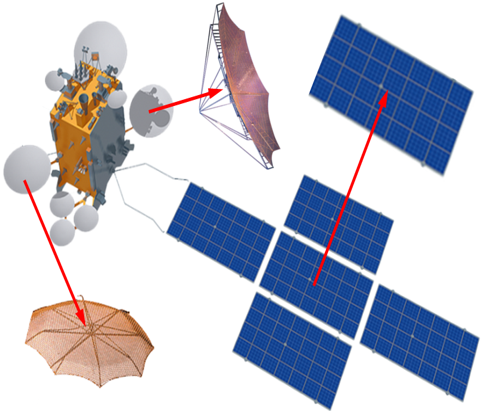
\includegraphics[width = 1\textwidth]{decomposition}
		\end{column}
		\begin{column}{0.5\textwidth}
			\centering
			% Определение стиля
			\tikzstyle{blockWide}=[rectangle, draw = black, fill = blue!20, rounded corners, text width = 20em, text centered, minimum height = 1.5em, drop shadow] % Блок
			\tikzstyle{blockWideC}=[blockWide, fill = red!20]
			\tikzstyle{arrow} = [draw, thick, color=black!90, -latex'] % Стрелка
			\scriptsize % Размер шрифта
			% Задание перменных
			\def\nodeDist{0.3cm} % Дистанция между узлами
			% Отрисовка блок-схемы
			\begin{tikzpicture}[scale = 1, transform shape]
				% Задание узлов		
				\node (modalTests) [blockWide] {Модальные испытания составных частей конструкции};
				\node (modelUpdating) [blockWide, below = \nodeDist of modalTests] {Коррекция расчетных моделей составных частей конструкции по результатам испытаний};
				\node (checkInfluence) [blockWide, below = \nodeDist of modelUpdating] {Освобождение закрепленных расчетных моделей составных частей конструкции};
				\node (buildRealModel) [blockWide, below = \nodeDist of checkInfluence] {Синтез расчетной модели полной конструкции из её составных частей};
				\node (buildMathModel) [blockWide, below = \nodeDist of buildRealModel] {Определение динамических характеристик полной расчетной модели};
				% Соединение узлов
				\draw [arrow] (modalTests.south) -- (modelUpdating.north);
				\draw [arrow] (modelUpdating.south) -- (checkInfluence.north);
				\draw [arrow] (checkInfluence.south) -- (buildRealModel.north);
				\draw [arrow] (buildRealModel.south) -- (buildMathModel.north);
			\end{tikzpicture}
		\end{column}
	\end{columns}
\end{frame}

\begin{frame}{Тестирование методики синтеза на расчетной модели космического аппарата (КА)}
	\begin{figure}
		\centering
		\includegraphics[width = 1\textwidth]{spacecraft-test-mesh}
	\end{figure}
	Число степеней свободы: $ 18714 $.
\end{frame}

\begin{frame}{Коррекция моделей составных частей тестового КА}
	\begin{figure}
		\centering
		\begin{subfigure}[t]{0.49\textwidth}
			\centering
			\includegraphics[width = \textwidth]{test-spacecraft-orbital-distribution}
			\caption{Орбитальный модуль} 
		\end{subfigure}
		\hfill
		\begin{subfigure}[t]{0.47\textwidth}
			\centering
			\includegraphics[height = \textwidth]{test-spacecraft-panel-distribution}
			\caption{Панели солнечных батарей} 
		\end{subfigure} 
		\caption{Изменения узловых жесткостей при коррекции составных частей}
	\end{figure}	
\end{frame}

\begin{frame}{Результаты синтеза глобальной модели КА}
	\begin{tblr}{
		colspec = {|X[c, -1]|X[c]|X[c]|X[c]|X[c]|},
		width = \textwidth, 
		hlines
	}
		\SetCell[r = 3]{c} № тона & \SetCell[c = 4]{c} Погрешность в частотах собственных колебаний, \% &&& \\
		& \SetCell[r = 2]{c} Без коррекции & \SetCell[c = 3]{c} Коррекция по девяти частотам && \\
		& & Панелей & Модуля & Панелей и модуля \\ \hline
		7 & -4.689 & -2.120 & -2.756 & -0.021 \\
		8 & -4.678 & -2.078 & -2.782 & -0.018 \\
		9 & -5.121 & -4.447 & -0.674 & 0.100  \\
		10 & -5.040 & -4.760 & -0.354 & -0.028 \\
		11 & -5.040 & -4.760 & -0.357 & -0.032 \\
		12 & -5.121 & -4.443 & -0.687 & 0.091 \\
		13 & -4.102 & -0.966 & -3.161 & 0.011 \\
		14 & -4.112 & -0.999 & -3.135 & 0.016 \\
		15 & -3.303 & -0.234 & -3.066 & -0.006 \\
	\end{tblr}
\end{frame}

\section{Программы для представления и обработки результатов модальных испытаний}

\begin{frame}{Программа для расчета обобщенных характеристик по результатам модальных испытаний}
	\begin{figure}
		\centering
		\includegraphics[width = 0.7\textwidth]{gencalc-interface}
	\end{figure}
\end{frame}

\begin{frame}{Программа для представления результатов модальных испытаний}
	\begin{figure}
		\centering
		\includegraphics[width = 0.8\textwidth]{analyzer-interface}
	\end{figure}
\end{frame}

\section{Программа для диагностирования дефектов конструкций по результатам испытаний}

\begin{frame}{Программа для диагностирования дефектов конструкций по результатам испытаний}
	\begin{figure}
		\centering
		\begin{subfigure}[t]{0.49\textwidth}
			\includegraphics[width = 0.75\textwidth]{distortion-airplane-forewing}
			\caption{Переднего горизонтального оперения}
		\end{subfigure}
		\hfill
		\begin{subfigure}[t]{0.49\textwidth}
			\includegraphics[width = 1\textwidth]{distortion-airplane-stabilizer} 
			\caption{Цельноповоротного стабилизатора}
		\end{subfigure}
    	\caption{Зазоры в узлах крепления оперения} 
	\end{figure}
\end{frame}

\section{Определение модальных характеристик по результатам акустических испытаний}

\begin{frame}{Определение модальных характеристик рефлектора по результатам акустических испытаний}
	\textbf{\underline{Принимаемые гипотезы}}:
	\begin{itemize}
		\item динамическая система является стационарной;
		\item исследуемый объект является наблюдаемым: расположение датчиков на конструкции позволяет однозначно идентифицировать формы колебаний, частоты которых лежат в интересующем диапазоне.
	\end{itemize}
	\begin{figure}
		\centering
		\begin{subfigure}[t]{0.49\textwidth}
			\includegraphics[width = 1\textwidth]{reflector-experiment}
			\caption{Рефлектор в акустической камере}
		\end{subfigure}
		\hfill
		\begin{subfigure}[t]{0.49\textwidth}
			\includegraphics[width = 1\textwidth]{reflector-sensors} 
			\caption{Расположение датчиков на поверхности рефлектора}
		\end{subfigure}
    	\caption{Проведение акустических испытаний} 
	\end{figure}
\end{frame}

\begin{frame}{Результаты определения динамических характеристик рефлектора методами операционного модального анализа}
	\centering
	\begin{tblr}{
		colspec = {|c|c|c|c||c|c|c|},
		hlines
	}
		\SetCell[r = 2]{c} Тон & \SetCell[c = 3]{c} Частота, Гц && & \SetCell[c = 3]{c} Логарифмический декремент && \\
		& SSI-COV & ERA & SSI-DD & SSI-COV & ERA & SSI-DD \\ \hline
		1 & 66.052 & 65.962 & 66.403 & 0.054 & 0.042 & 0.045 \\
		2 & 91.287 & 90.910 & 91.843 & 0.030 & 0.052 & 0.042 \\
		3 & 102.540 & --- & --- & 0.056 & --- & --- \\
		4 & 114.770 & --- & --- & 0.063 & --- & --- \\
		5 & 122.370 & --- & --- & 0.094 & --- & --- \\
		6 & 127.850 & --- & --- & 0.049 & --- & --- \\
	\end{tblr}
\end{frame}

\section{Определение модальных характеристик по результатам летных испытаний}

\begin{frame}{Определение модальных характеристик по результатам летных испытаний}
	\begin{block}{Методика определения критической скорости флаттера}
		\begin{itemize}
			\item выход летательного аппарата на исследуемый скоростной режим;
			\item задание генератором сигналов в систему управления; 
			\item передача системой управления воздействий отклоняемым поверхностям;
			\item регистрация колебаний тензодатчиками и акселерометрами до полного завершения переходных процессов;
			\item обобщение и обработка результатов измерений на различных скоростях полета.
		\end{itemize}
	\end{block}
	\begin{block}{Типы возбуждения в ходе полета}
		\begin{itemize}
			\item развертка сигнала по частоте; 
			\item кратковременное гармоническое воздействие на исследуемой частоте; 
			\item неспокойная атмосфера.
		\end{itemize}
	\end{block}
\end{frame}

\begin{frame}{Результаты обработки летных испытаний Су-30}
	\begin{figure}
		\begin{subfigure}[b]{0.49\textwidth}
			\centering
	     	\includegraphics[width = 1\textwidth]{flight-decrements-2} 
	     	\caption{Полет № 1}
	    \end{subfigure}
    	\hfill
	    \begin{subfigure}[b]{0.49\textwidth}
			\centering
			\includegraphics[width = 1\textwidth]{flight-decrements-1}
			\caption{Полет № 2}
	    \end{subfigure}
    	\caption{Кривые зависимости логарифмических декрементов от скорости полета}
	\end{figure}
\end{frame}

\section{Решение практических задач коррекции расчетных моделей}

\section{Коррекция расчетной модели динамически-подобной модели самолета Ту-204}

\begin{frame}{Коррекция расчетной модели динамически-подобной модели самолета Ту-204}
	\begin{figure}
		\begin{subfigure}[t]{0.49\textwidth}
			\centering
	     	\includegraphics[width = 1\textwidth]{tu-204-experiment} 
	     	\caption{Упругое вывешивание модели}
	    \end{subfigure}
    	\hfill
	    \begin{subfigure}[t]{0.49\textwidth}
			\centering
			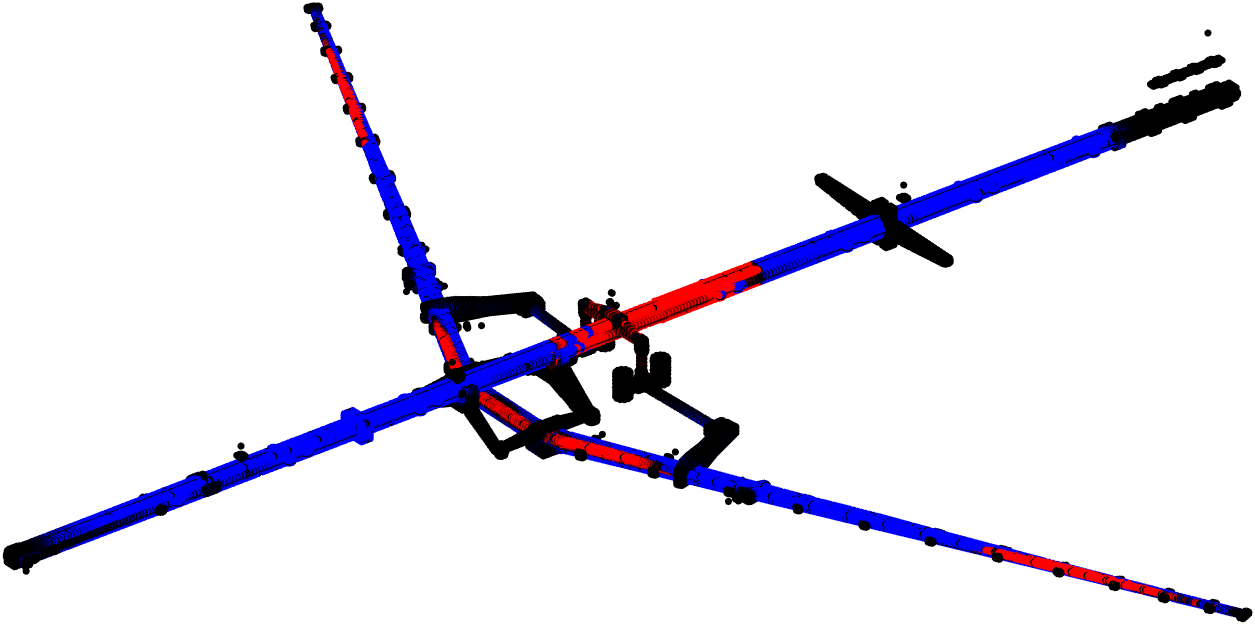
\includegraphics[width = 1\textwidth]{tu-204-coeffs-6}
			\caption{Изменение узловых жесткостей}
	    \end{subfigure}
	    \caption{Динамически-подобная модель самолета Ту-204}
	\end{figure}
\end{frame}

\begin{frame}{Результаты применения метода коррекции} 
	\resizebox{\textwidth}{!}{%
	\begin{tblr}
	{
		colspec = {|c|c|c|c|c|c|c|c|c|c|}, 
		hlines
	}
   		\SetCell[r = 3]{c} Тон & \SetCell[c = 2]{c} Частоты, Гц && \SetCell[c = 7]{c} Погрешность до и после коррекции, \%  \\
	   	& \SetCell[r = 2]{c} Эксперимент & \SetCell[r = 2]{c} {Исходная \\ модель} & \SetCell[r = 2]{c} До & \SetCell[c = 6]{c} После \\ 
   		& & & & 1 & 2 & 3 & 4 & 5 & 6 \\ \hline
		СИКр1 & 3.44 & 3.49 & 1.5 & 0.0 & 0.0 & 0.0 & 0.0 & 0.0 & 0.0 \\
		АСИКр1 & 4.87 & 4.96 & 1.7 & -0.6 & 0.0 & 0.0 & 0.0 & 0.0 & 0.0 \\
		ГИФ1 & 5.44 & 5.73 & 5.3 & 4.7 & 4.7 & 0.0 & 0.0 & 0.0 & 0.0 \\ 
		ВИФ1 & 5.73 & 5.97 & 4.2 & 3.5 & 3.3 & 2.6 & 0.0 & 0.0 & 0.0 \\
		СИКр2 & 9.30 & 9.13 & -1.8 & -4.4 & -3.2 & -3.9 & -4.4 & 0.0 & 0.0 \\
		ВИФ2 & 14.18 & 14.77 & 4.2 & 3.7 & 3.8 & 3.4 & 2.0 & 3.3 & 0.0 \\
	\end{tblr} }
	\footnotetext[1]{Cимметричный изгиб крыла I тона}
	\footnotetext[2]{Антисимметричный изгиб крыла I тона}
	\footnotetext[3]{Горизонтальный изгиб фюзеляжа I тона}
	\footnotetext[4]{Вертикальный изгиб фюзеляжа I тона}
	\footnotetext[5]{Симметричный изгиб крыла II тона}
	\footnotetext[6]{Вертикальный изгиб фюзеляжа II тона}
\end{frame}

\section{Синтез имитационной модели каркаса зонтичной антенны космического аппарата}

\begin{frame}{Синтез имитационной модели каркаса зонтичной антенны космического аппарата}
	\begin{figure}
		\centering
		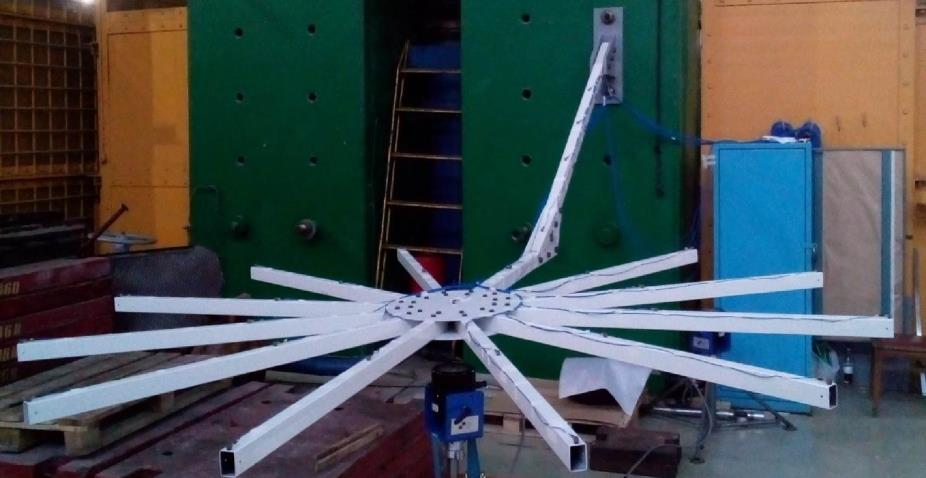
\includegraphics[width = 0.9\linewidth]{simsat-assembly}
		\caption{Общий вид имитационной модели каркаса зонтичной антенны в сборе} 
	\end{figure}
\end{frame}

\begin{frame}{Составные части имитационной модели}
	\begin{figure}
		\centering
		\begin{subfigure}[t]{0.48\textwidth}
			\centering
			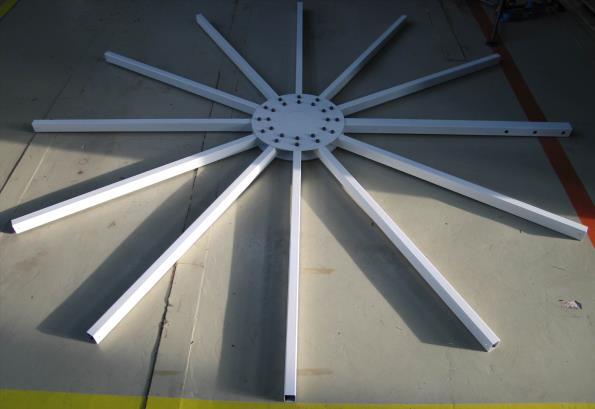
\includegraphics[width = \textwidth]{simsat-antenna}
			\caption{Зонтичный каркас}
		\end{subfigure}
		\hfill
		\begin{subfigure}[t]{0.48\textwidth}
			\centering
			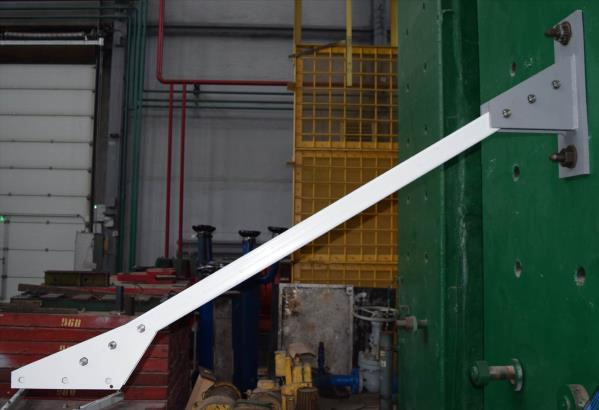
\includegraphics[width = \textwidth]{simsat-handle}
			\caption{Штанга}
		\end{subfigure}	
		\caption{Составные части модели каркаса зонтичной антенны}
	\end{figure}
\end{frame}

\begin{frame}{Результаты применения методики синтеза} 
	\centering
	\begin{tblr}
	{
		colspec = {|c|c|c|c|}, 
		width = \textwidth, 
		hlines
	}
		\SetCell[r = 3]{c} Тон & \SetCell[c = 3]{c} {Погрешность относительно эксперимента \\ до и после коррекции  моделей составных частей, \%} \\ \cline{2-4} 
		& \SetCell[r = 2]{c} До коррекции & \SetCell[c = 2]{c} После коррекции & \\ \cline{3-4} 
		& & Коррекция штанги & {Коррекция штанги и \\ антенны} \\ \hline
		1 & 1.84 & 0.70 & 0.70 \\ 
	    2 & 3.88 & 0.33 & 0.40 \\ 
	    3 & 3.19 & 1.24 & 1.24 \\ 
    	4 & 2.13 & 1.18 & 1.18 \\ 
	    5 & 2.25 & 2.73 & 1.95 \\ 
	    6 & 3.55 & 3.48 & 3.41 \\ 
    	7 & 3.78 & 3.64 & 3.64 
	\end{tblr}
\end{frame}

\subsection{Коррекция расчетной модели отъемной части крыла изделия С-70}

\begin{frame}{Коррекция расчетной модели отъемной части крыла изделия С-70}
	\begin{figure}
		\begin{subfigure}[b]{0.38\textwidth}
			\centering
	     	\includegraphics[width = 1\textwidth]{wing-experiment} 
	     	\caption{Консоль крыла на подвеске}
	    \end{subfigure}
    	\hfill
	    \begin{subfigure}[b]{0.61\textwidth}
			\centering
			\includegraphics[width = 1\textwidth]{wing-coeffs-5}
			\caption{Распределение изменений узловых жесткостей}
	    \end{subfigure}
	    \caption{Композитная консоль крыла изделия С-70}
	\end{figure}
\end{frame}

\begin{frame}{Результаты коррекции композитной консоли крыла} 
	\centering
	\begin{tblr}{
		colspec = {|c|c|c|c|c|c|c|c|c|}, 
		width = \textwidth, 
		hlines
	}
		\SetCell[r = 3]{c} Тон & \SetCell[c = 2]{c} Приведенная частота && \SetCell[c = 6]{c} Погрешность до и после коррекции, \% \\
		& \SetCell[r = 2]{c} Эксперимент & \SetCell[r = 2]{c} {Исходная \\ модель} & \SetCell[r = 2]{c} До & \SetCell[c = 5]{c}После \\
		& & & & 1 & 2 & 3 & 4 & 5 \\ \hline
		1 & 1.00 & 1.51 & 50.7 & 0.0 & 0.0 & 0.0 & 0.0 & 0.0 \\ 
		2 & 2.28 & 3.18 & 39.5 & -7.4 & 0.0 & 0.0 & 0.0 & 0.0 \\ 
		3 & 3.37 & 4.13 & 22.6 & -18.6 & -13.8 & 0.0 & 0.0 & 0.0 \\ 
		4 & 3.95 & 4.82 & 21.8 & -19.1 & -17.8 & -8.2 & 0.0 & 0.0 \\ 
		5 & 4.87 & 6.15 & 26.2 & -16.2 & -21.8 & -2.6 & -4.4 & 0.0 \\ 
	\end{tblr}
\end{frame}

\begin{frame}{Сопоставление форм колебаний до и после коррекции}
	\begin{block}{Критерий модального соответствия (MAC-критерий)}
		\begin{equation}
			\mathrm{MAC}_{i, j} = \frac{(\mat{u}_i ^ \intercal \cdot \mat{v}_j) ^ 2}{(\mat{u}_i ^ \intercal \cdot \mat{u}_i) (\mat{v}_j ^ \intercal \cdot \mat{v}_j)}, 
		\end{equation}
		где $ \mat{u}_i $ и $ \mat{v}_j $~---~формы колебаний до и после коррекции; $ i, j = 1 \hdots n $.
	\end{block}
	\vspace{-0.5em}
	\begin{columns}
		\begin{column}{0.49\textwidth}
			\centering
			\begin{figure}
				\includegraphics[width=1\textwidth]{wing-MAC}
			\end{figure}
		\end{column}
		\begin{column}{0.4\textwidth}
			\centering
			\begin{figure}
				\includegraphics[width=1\textwidth]{wing-initial-mode-1} \\ \vspace{0.2em}
				\includegraphics[width=1\textwidth]{wing-initial-mode-2} \\ \vspace{0.2em}
				\includegraphics[width=1\textwidth]{wing-initial-mode-3} \\ \vspace{0.2em}
				\includegraphics[width=1\textwidth]{wing-initial-mode-4}
			\end{figure}
		\end{column}
	\end{columns}
\end{frame}

\subsection{Коррекция расчетной модели гирдера для модульных секций накопителя ЦКП <<СКИФ>>}

\begin{frame}{Коррекция расчетной модели гирдера для модульных секций накопителя ЦКП <<СКИФ>>}
	\begin{figure}
		\begin{subfigure}[b]{0.49\textwidth}
			\centering
	     	\includegraphics[width = 1\textwidth]{girder-full-system} 
	     	\caption{Совместная геометрическая модель гирдера и магнитов}
	    \end{subfigure}
    	\hfill
	    \begin{subfigure}[b]{0.49\textwidth}
			\centering
			\includegraphics[width = 1\textwidth]{girder-experiment}
			\caption{Модальные испытания гирдера без магнитов}
	    \end{subfigure}
	    \caption{Гирдер для модульных секций накопителя}
	\end{figure}
\end{frame}

\begin{frame}{Результаты коррекции расчетной модели гирдера}
	\textbf{\underline{Последовательность коррекции}}
	\begin{enumerate}
		\item Уточнение упругих характеристик основания ($ 2 $ минуты).
		\item Коррекция четырех упругих горизонтальных тонов ($ 7 $ минут).
		\item Коррекция двух упругих вертикальных тонов ($ 1 $ минута).
		\item Коррекция всех шести упругих тонов ($ 4 $ минуты).
	\end{enumerate}
	\vfill
	\centering
	\begin{tblr}{
		colspec = {|X[c, -1]|X[c]|X[c]|X[c]|X[c]|}, 
		width = \textwidth, 
		hlines
	}
		\SetCell[r = 2]{c} Тон & \SetCell[c = 2]{c} Частота, Гц && \SetCell[c = 2]{c} Погрешность, \% \\
		& Эксперимент & Исходная модель & До коррекции & После коррекции \\ \hline
		6 & 119.51 & 135.08 & 13.03 & \SetCell[r = 6]{c} \textbf{0.00} \\
		7 & 140.97 & 146.46 & 3.89 &  \\
		8 & 148.13 & 160.07 & 8.06 &  \\
		9 & 189.65 & 210.48 & 10.98 & \\
		10 & 197.53 & 214.18 & 8.43 & \\
		11 & 242.24 & 253.51 & 4.65 & \\
	\end{tblr}
\end{frame}

\begin{frame}{Результаты коррекции расчетной модели гирдера}
	\begin{figure}[!htb]
		\centering
		\begin{subfigure}[t]{0.49\textwidth}
			\centering
			\includegraphics[width = \textwidth]{girder-coeffs-0-6} 
			\caption{Относительно исходной модели} 
		\end{subfigure}
		\hfill
		\begin{subfigure}[t]{0.49\textwidth}
			\centering
			\includegraphics[width = \textwidth]{girder-coeffs-1-6}
			\caption{Относительно коррекции по одной частоте} 
		\end{subfigure}	
		\caption{Изменения узловых жестокостей до и после коррекции КЭ-модели} 
	\end{figure}
\end{frame}